%----------------------------------------------------------------------------
\chapter{Experimental results}
\label{chap:experimental}
%----------------------------------------------------------------------------

\section{YOLO}

Initially I wanted to use YOLOv4~\cite{Bochkovskiy2020YOLOv4OS} as the sole
detection algorithm. YOLO is indeed realtime however it only provides 2D
bounding boxes of the detections which is not enough when we need to mask the
depth map with an instance segmentation.

\begin{figure}[!ht]
	\centering
	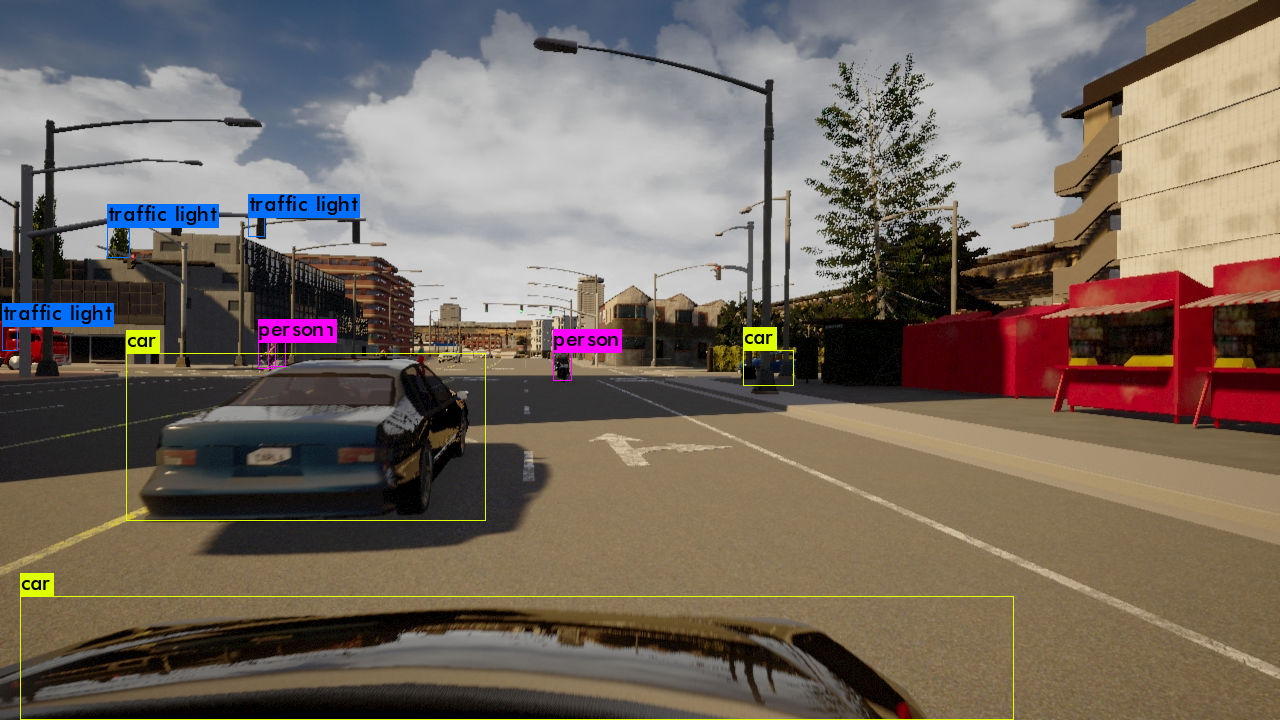
\includegraphics[width=150mm, keepaspectratio]{figures/yolo.jpg}
	\caption{YOLOv4 under evaluation}
	\label{fig:yolo}
\end{figure}

\section{Tracking}

As mentioned previously it is essential to track objects throught time. I tested
Deep SORT~\cite{Wojke2018deep} algorithm which is an improvement over Simple
Online and Realtime Tracking (SORT)~\cite{Wojke2017simple}. This building block
ended upnot being in the detector however a following version will certainly
need a tracker method. 

Deep SORT also works with Kalman filters and it needs detection instances to
predict identites over time. Each bounding box is provided to the tracker which
then creates a signature of the detection based on it's pixel values and then
calculates distances with other previously dtected object from a dictionary. A
single counter is incremented for each new object that couldn't be correlated
with the previously detected objects.

I evaluated test using YOLOv4 as the detector. Results of a test video can be seen in
\autoref{fig:deepsort}

\begin{figure}[!ht]
	\centering
	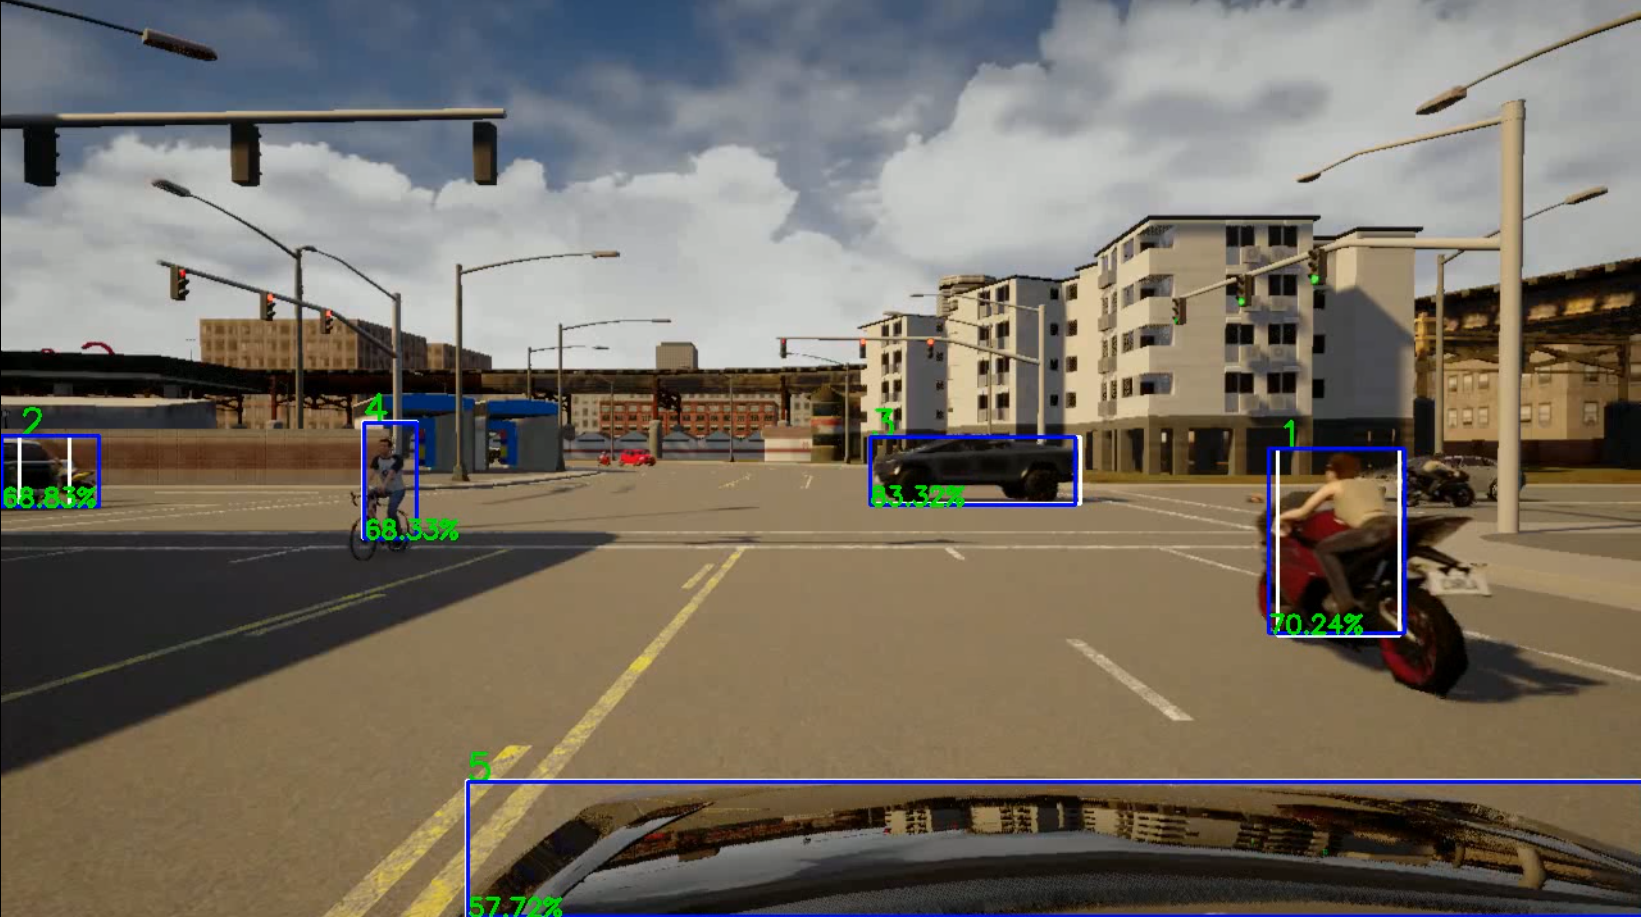
\includegraphics[width=150mm, keepaspectratio]{figures/deepsort.png}
	\caption{Screenshot during a video being processed by the tracker.}
	\label{fig:deepsort}
\end{figure}

\section{Lane detection}

When I experimented with lane detection I once tried to use a neural network for
the task. Hough transform and sliding window technique could have been enough
but I was curious of the accuracy on the simulator. 

"Towards End-to-End Lane Detection: an Instance Segmentation
Approach"~\cite{DBLP:journals/corr/abs-1903-11027} is a neural network that
basically works as an edge detector that is directed towards the vanishing point
in the image. Note the if the network had been trained it might have yielded
better results! In the results of the original paper the results were better but
the training data was specific to a certain road.

\begin{figure}[!ht]
	\centering
	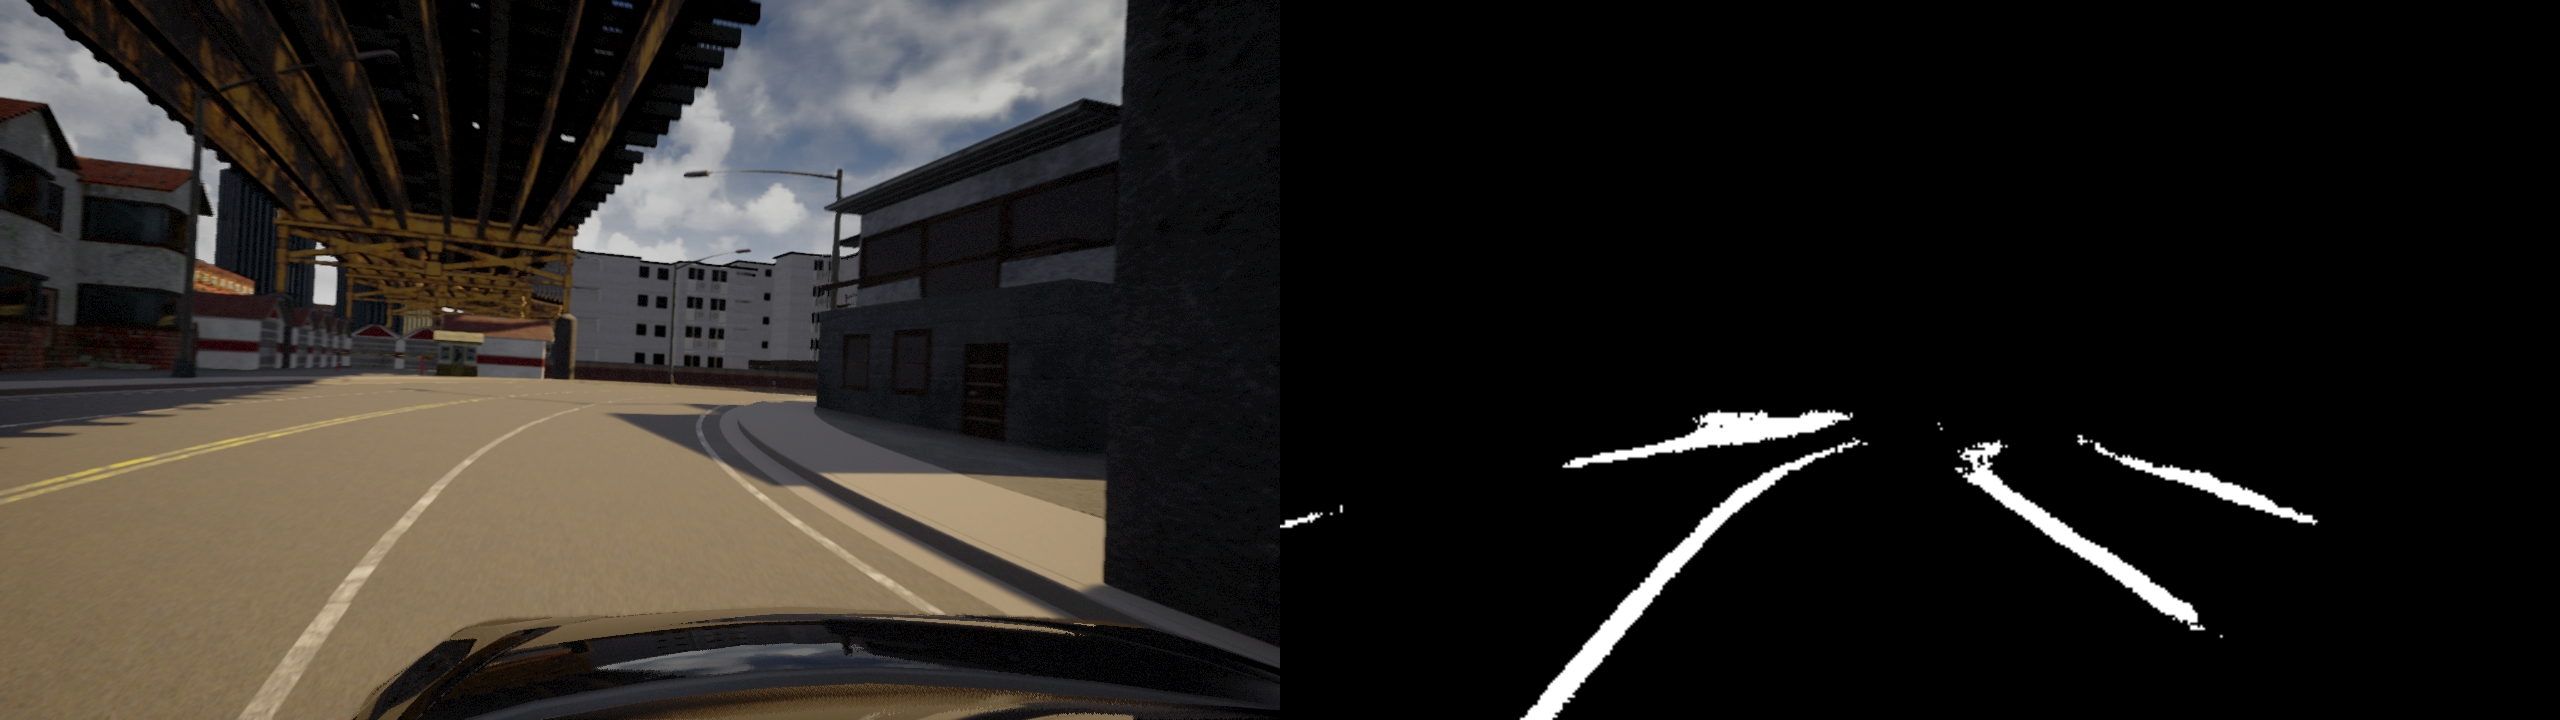
\includegraphics[width=150mm, keepaspectratio]{figures/lanedet.png}
	\caption{Lane detection performed well without training}
	\label{fig:lanedet}
\end{figure}

\section{Orientation estimation}
As mentioned earlier as an essential imporvement over the current algorithm. I
evaluated two approaches. The first approach is direct 3D bounding box detection
the second is keypoint detection.

\subsection{3D Bounding box detection}

Direct orientation estimation would be an important part of the detector as
mentioned previously in improvements. Before implementing the detector I tried a
CNN implementation\footnote{3D Bounding Box implementation
\url{https://github.com/skhadem/3D-BoundingBox}} based on the paper "3D Bounding
Box Estimation Using Deep Learning and
Geometry"~\cite{DBLP:journals/corr/MousavianAFK16}. This network works similarly
to landmark detection but it adds geometric constraints to regress the
orientation of the bounding boxes.

\begin{figure}[!ht]
	\centering
	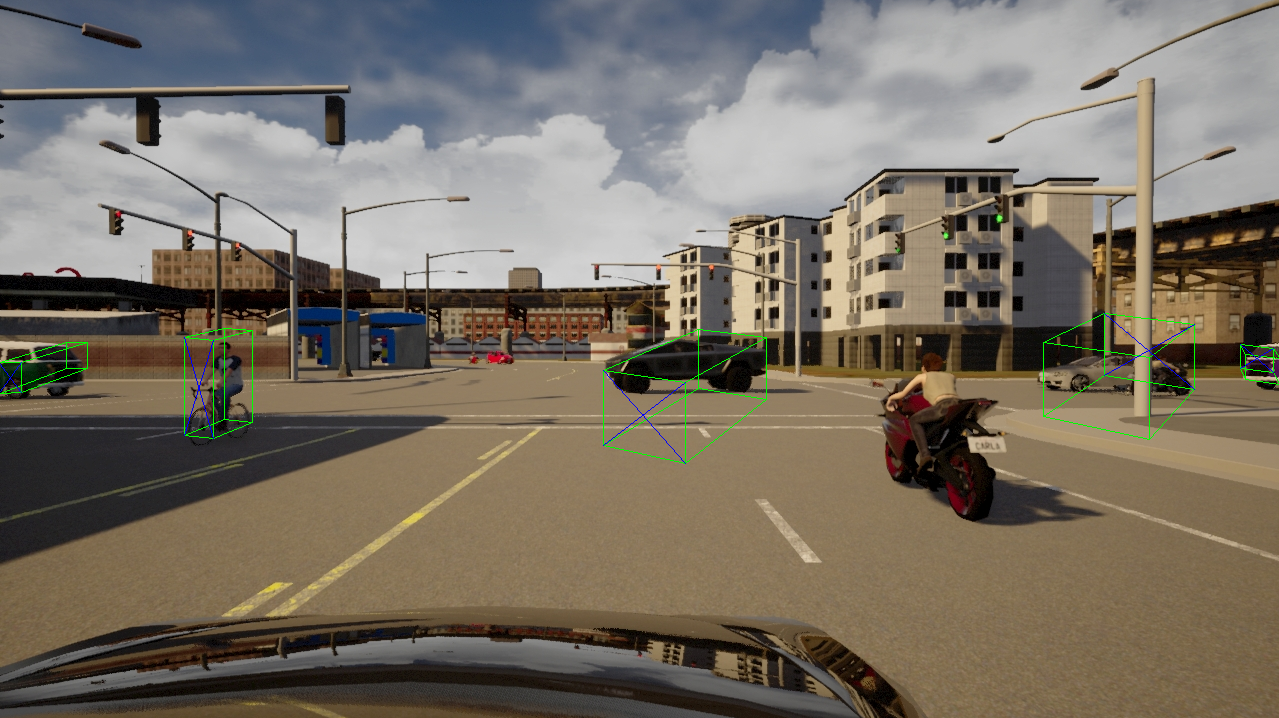
\includegraphics[width=150mm, keepaspectratio]{figures/boundingbox.png}
	\caption{Bounding box detection performed poorly. Note, that YOLOv3 missed the motorcycle, thus it is not predicted}
	\label{fig:boundingbox}
\end{figure}

\subsection{Keypoint detection}
After the previous approach failed next idea was that we could derive the
orientation of the vehicles if we knew the position of it's keypoints/landmarks
in the images. After some research I found a research developed at Google AI
"Discovery of Latent 3D Keypoints via End-to-end Geometric Reasoning" or
KeypointNet~\cite{suwajanakorn_discovery_2018}. 

The netowrk performed poorly on CARLA vehicles. I tried with and without
instance segmentation but the results seemed independent.

\begin{figure}[!ht]
	\centering
	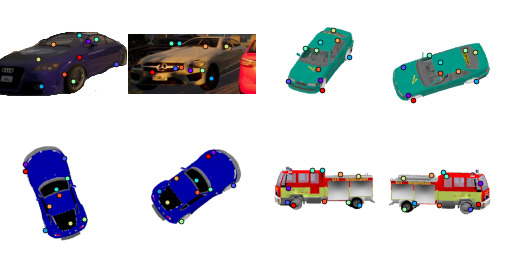
\includegraphics[width=150mm, keepaspectratio]{figures/keypoints.jpg}
	\caption{Keypoint detection on CARLA vehicles was inaccurate}
	\label{fig:keypoints}
\end{figure}

\begin{figure}[!ht]
	\centering
	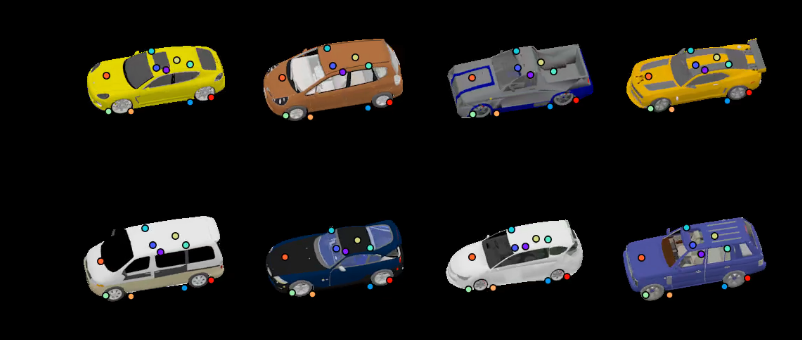
\includegraphics[width=150mm, keepaspectratio]{figures/keypointnet.png}
	\caption{Expected results (from \url{https://keypointnet.github.io/})}
	\label{fig:keypointnet}
\end{figure}